%%%%%%%%%%%%%%%%%%%%%%%%%%%%%%%%%%%%%%%%%
% Jacobs Landscape Poster
% LaTeX Template
% Version 1.0 (29/03/13)
%
% Created by:
% Computational Physics and Biophysics Group, Jacobs University
% https://teamwork.jacobs-university.de:8443/confluence/display/CoPandBiG/LaTeX+Poster
% 
% Further modified by:
% Nathaniel Johnston (nathaniel@njohnston.ca)
%
% This template has been downloaded from:
% http://www.LaTeXTemplates.com
%
% License:
% CC BY-NC-SA 3.0 (http://creativecommons.org/licenses/by-nc-sa/3.0/)
%
%%%%%%%%%%%%%%%%%%%%%%%%%%%%%%%%%%%%%%%%%

%----------------------------------------------------------------------------------------
%	PACKAGES AND OTHER DOCUMENT CONFIGURATIONS
%----------------------------------------------------------------------------------------

\documentclass[final]{beamer}
\usepackage[utf8]{inputenc}

\usepackage[scale=1.24]{beamerposter} % Use the beamerposter package for laying out the poster

\usetheme{confposter} % Use the confposter theme supplied with this template

\setbeamercolor{block title}{fg=ngreen,bg=white} % Colors of the block titles
\setbeamercolor{block body}{fg=black,bg=white} % Colors of the body of blocks
\setbeamercolor{block alerted title}{fg=white,bg=dblue!70} % Colors of the highlighted block titles
\setbeamercolor{block alerted body}{fg=black,bg=dblue!10} % Colors of the body of highlighted blocks
% Many more colors are available for use in beamerthemeconfposter.sty

%-----------------------------------------------------------
% Define the column widths and overall poster size
% To set effective sepwid, onecolwid and twocolwid values, first choose how many columns you want and how much separation you want between columns
% In this template, the separation width chosen is 0.024 of the paper width and a 4-column layout
% onecolwid should therefore be (1-(# of columns+1)*sepwid)/# of columns e.g. (1-(4+1)*0.024)/4 = 0.22
% Set twocolwid to be (2*onecolwid)+sepwid = 0.464
% Set threecolwid to be (3*onecolwid)+2*sepwid = 0.708

\newlength{\sepwid}
\newlength{\onecolwid}
\newlength{\twocolwid}
\newlength{\threecolwid}
\setlength{\paperwidth}{48in} % A0 width: 46.8in
\setlength{\paperheight}{36in} % A0 height: 33.1in
\setlength{\sepwid}{0.024\paperwidth} % Separation width (white space) between columns
\setlength{\onecolwid}{0.22\paperwidth} % Width of one column
\setlength{\twocolwid}{0.464\paperwidth} % Width of two columns
\setlength{\threecolwid}{0.708\paperwidth} % Width of three columns
\setlength{\topmargin}{-0.5in} % Reduce the top margin size
%-----------------------------------------------------------

\usepackage{graphicx}  % Required for including images

\usepackage{booktabs} % Top and bottom rules for tables

%----------------------------------------------------------------------------------------
%	TITLE SECTION 
%----------------------------------------------------------------------------------------

\title{Secure Computations in Decentralized Environments \\based on Smart Contracts and Intel SGX} % Poster title

\author{Michał Król, Adrian-Cristian Nicolaescu, Sergi Reñé, Onur Ascigil, Ioannis Psaras, David Oran, Dirk Kutscher} % Author(s)

\institute{University College London, Network Systems Research \& Design, Huawei} % Institution(s)

%----------------------------------------------------------------------------------------

\begin{document}

\addtobeamertemplate{block end}{}{\vspace*{2ex}} % White space under blocks
\addtobeamertemplate{block alerted end}{}{\vspace*{2ex}} % White space under highlighted (alert) blocks

\setlength{\belowcaptionskip}{2ex} % White space under figures
\setlength\belowdisplayshortskip{2ex} % White space under equations

\begin{frame}[t] % The whole poster is enclosed in one beamer frame

\begin{columns}[t] % The whole poster consists of three major columns, the second of which is split into two columns twice - the [t] option aligns each column's content to the top

\begin{column}{\sepwid}\end{column} % Empty spacer column

\begin{column}{\onecolwid} % The first column

%----------------------------------------------------------------------------------------
%	MOTIVATION
%----------------------------------------------------------------------------------------

\begin{alertblock}{Motivation}
There is a rising need for distributed computation. Currently everything is done in the cloud, but:
\begin{itemize}
\item Privacy issues.
\item High execution cost.
\item High delay.
\end{itemize}
There is a lot of unused computational power at the edge, but:
\begin{itemize}
 \item Nodes do not trust one another.
 \item There are no easy mechanisms to prove result validity.
 \item There are no simple payment mechanisms. 
\end{itemize}


\end{alertblock}

\begin{block}{Actors}
 \begin{itemize}
  \item[] 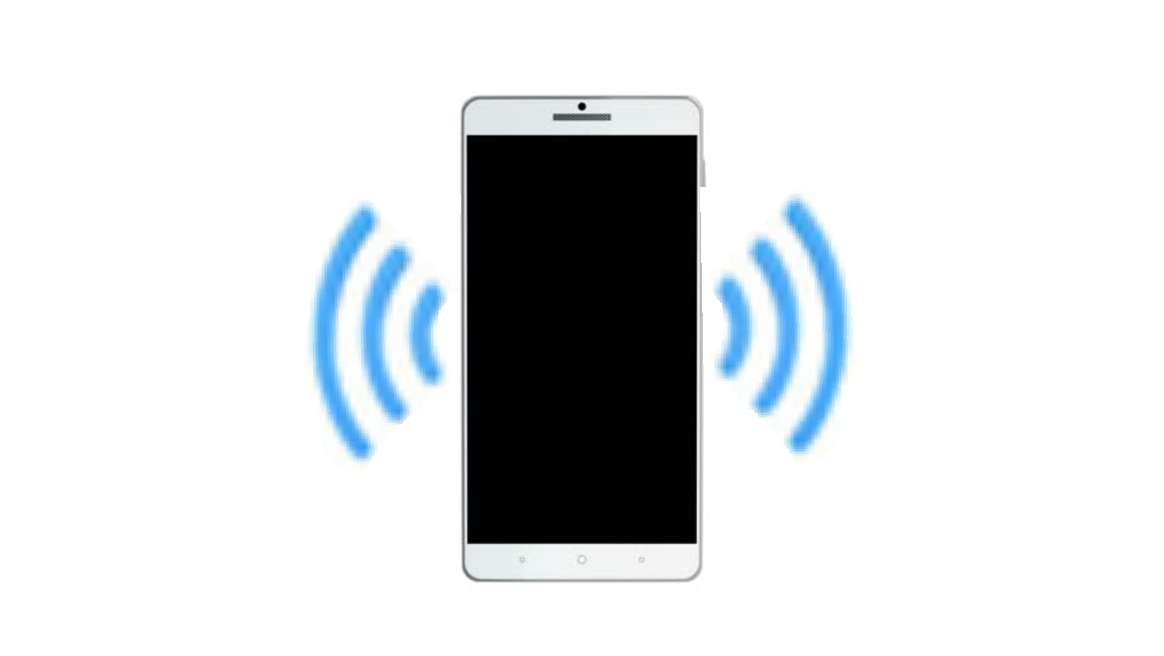
\includegraphics[width=0.09\linewidth]{img/user} \textbf{Requestor} - submits tasks to the system
  \item[] 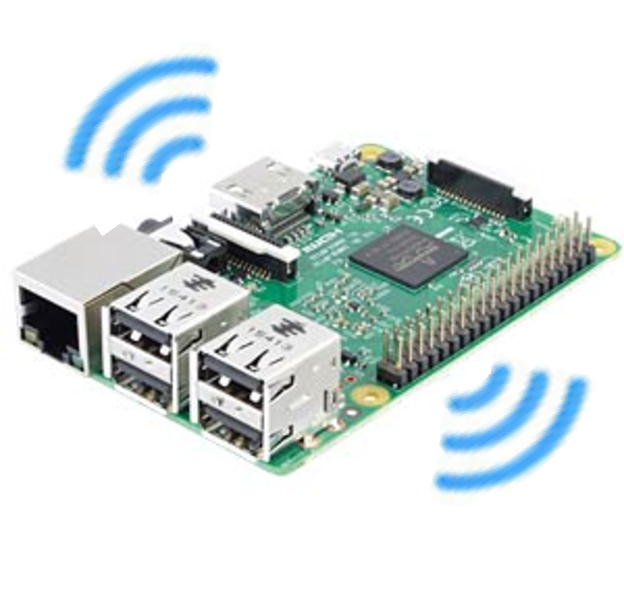
\includegraphics[width=0.07\linewidth]{img/pi} \textbf{Execution Node} - executes tasks
 \end{itemize}

\end{block}



%----------------------------------------------------------------------------------------
%	INTRODUCTION
%----------------------------------------------------------------------------------------

\begin{block}{Technologies}
\textbf{Intel SGX}
  \begin{itemize}
    \item Creates \emph{enclaves} that are protected by the CPU against access from other OS/Hypervisor
    \item Remote Attestation Protocol
    \begin{itemize}
      \item Verifies the code running on a remote node
      \item Allows secure communication with the enclave
    \end{itemize}
  \end{itemize}
  
\textbf{Blockchain}
  \begin{itemize}
  \item Immutable, Distributed Ledger
  \item Smart Contracts
    \begin{itemize}
      \item Allow to logic on top of a blockchain
      \item Turing complete language (Solidity)
      \item Submitted data is publicly visible
    \end{itemize}
  \end{itemize}
\end{block}

%----------------------------------------------------------------------------------------

\end{column} % End of the first column

\begin{column}{\sepwid}\end{column} % Empty spacer column

\begin{column}{\twocolwid} % Begin a column which is two columns wide (column 2)

\begin{figure}
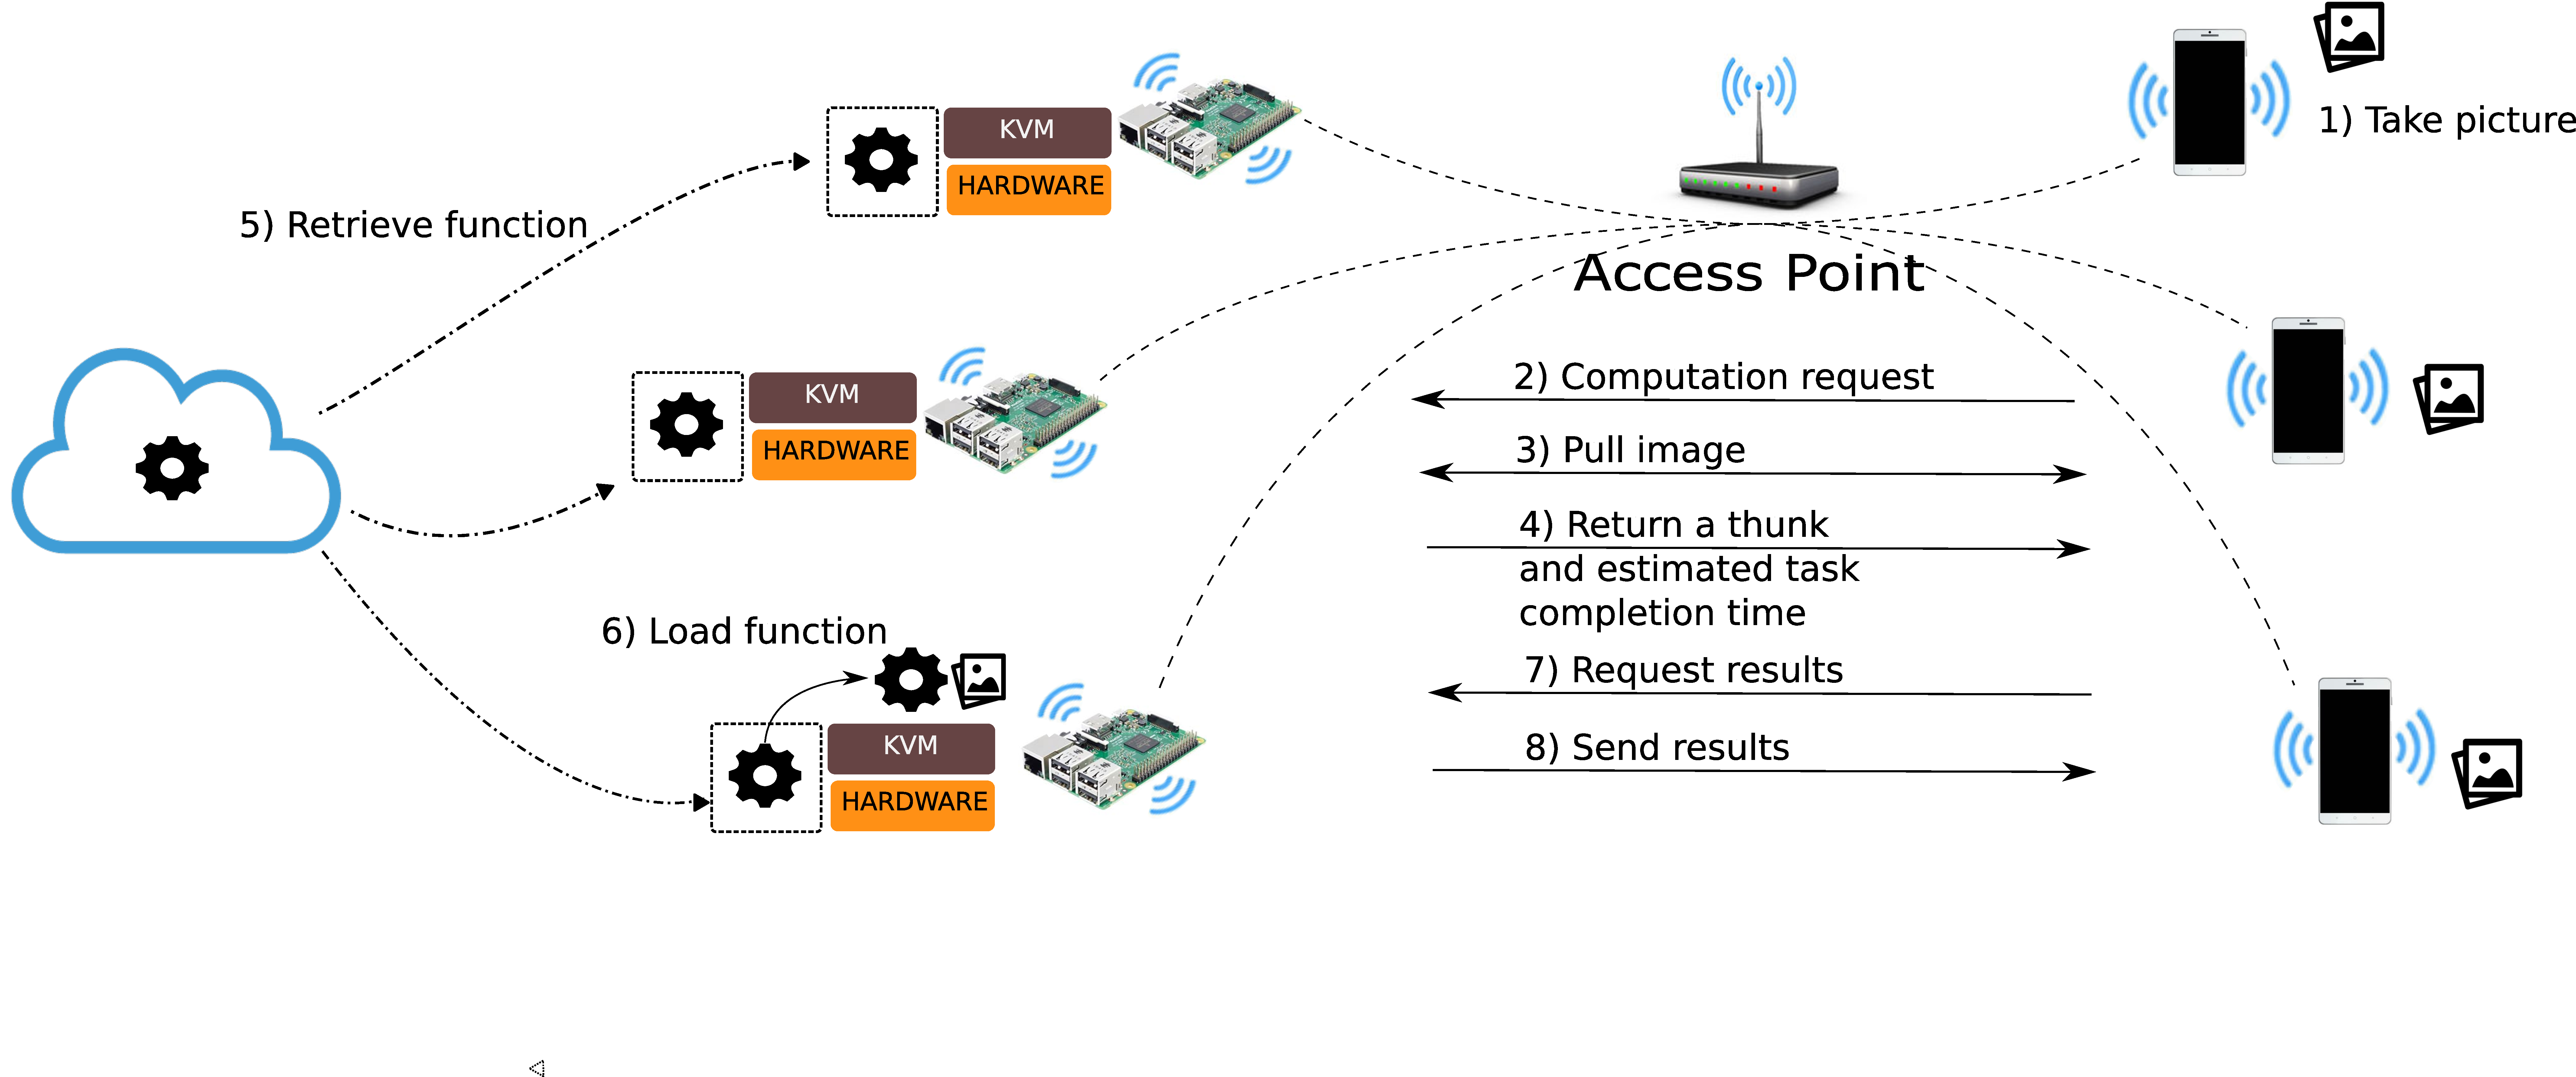
\includegraphics[width=1\linewidth]{img/scenario}
\end{figure}

\noindent\rule{55cm}{0.4pt}


\end{column} % End of the second column

\begin{column}{\sepwid}\end{column} % Empty spacer column

\begin{column}{\onecolwid} % The third column

%----------------------------------------------------------------------------------------
%	CONCLUSION
%----------------------------------------------------------------------------------------

\begin{block}{Design Goals}
\begin{itemize}
 \item \textbf{Openness} - everyone can join the system and submit or execute tasks. 
 \item \textbf{Incentives} - \emph{Execution Nodes} are paid for their work. 
 \item \textbf{Result Integrity} - \emph{Requestors} are sure that the returned result is correct.
 \item \textbf{Input/Output Privacy} - input parameters and result data are visible only to the \emph{Requestor} and hidden from the \emph{Execution Node}. 
\end{itemize}

\end{block}


%----------------------------------------------------------------------------------------
%	RESULTS
%----------------------------------------------------------------------------------------

\setbeamercolor{block alerted title}{fg=black,bg=norange} % Change the alert block title colors
\setbeamercolor{block alerted body}{fg=black,bg=white} % Change the alert block body colors

\begin{alertblock}{Results}

\begin{itemize}
\item A prototype running on Ethereum Test Network. 
\item Orders of magnitude less overhead than the State of the Art.
\item Fully automated payments and result verification. 
\item Operating cost lower than $1\$$.
\item No 3rd parties involved. 
\item Secure against rational attacker. 
\end{itemize}

\end{alertblock}

%----------------------------------------------------------------------------------------
%	CONCLUSION
%----------------------------------------------------------------------------------------

\begin{block}{Current Limitations}
\begin{itemize}
 \item Delay imposed by the blockchain (few minutes).
 \item Function size limited to 100MB. 
 \item Requires Intel hardware. 
 \item Not secure against arbitrary attacker. 
\end{itemize}

\end{block}

%----------------------------------------------------------------------------------------

\end{column} % End of the third column

\end{columns} % End of all the columns in the poster

\end{frame} % End of the enclosing frame

\end{document}
